\documentclass[a4paper]{article}

\usepackage{INTERSPEECH2019}
\usepackage{tabu}
\usepackage{booktabs}
\usepackage{color}
\usepackage{pifont}
% Please add the following required packages to your document preamble:
\usepackage{multirow}
\usepackage{graphicx}
\usepackage{comment}
%%%%%%%%%%%%%%%%%%%%%%%%%%%%%%%%%%%%%%%%%%%%%%%%%%%%%%%%%%%
%%%%%%%% SHOW COMMENTS
\newcommand{\Soo}[1]{\textcolor{magenta}{[Soo: #1]}}
\newcommand{\Vijay}[1]{\textcolor{green}{[Vijay: #1]}}
\newcommand{\Amber}[1]{\textcolor{red}{[Amber: #1]}}
%%%%%%%%%%%%%%%%%%%%%%%%%%%%%%%%%%%%%%%%%%%%%%%%%%%%%%%%%%%
%%%%%%%% DON'T SHOW COMMENTS
% \newcommand{\Soo}[1]{}
% \newcommand{\Vijay}[1]{}
% \newcommand{\Amber}[1]{}
%%%%%%%%%%%%%%%%%%%%%%%%%%%%%%%%%%%%%%%%%%%%%%%%%%%%%%%%%%%

% \doublespacing
\usepackage{amsmath}
\DeclareMathOperator{\Tr}{\textbf{Tr}}
\newcommand{\etal}{\textit{et al}.}

\title{Voice Quality and Change in Entropy for Sleepiness Estimation}
\name{Vijay Ravi, Soo Jin Park, Amber Afshan and Abeer Alwan}
%The maximum number of authors in the author list is twenty. If the number of contributing authors is more than twenty, they should be listed in a footnote or in acknowledgement section, as appropriate.
\address{Electrical and Computer Engineering Department, University of California Los Angeles, USA}
\email{vijaysumaravi@ucla.edu, sj.park@ucla.edu, amberafshan@g.ucla.edu, alwan@g.ucla.edu}

\begin{document}

\maketitle
% 
\begin{abstract}
Sleepiness monitoring and prediction has many potential applications, such as being a safety feature in driver-assistance systems. In this study, we address the ComparE 2019 Continuous Sleepiness task of estimating the sleepiness degree from speech signals. Voice quality features and between-frame changes in entropy are proposed to capture acoustic characteristics related to the sleepiness state of a speaker. Voice quality is often associated with a speaker's physical and emotional state. Frame-level changes in entropy can be considered as indirect measures of speaking rate. We also propose a multi-level prediction strategy. In the first level, a support vector classifier was trained using a vector of entropy statistics. For best results, utterances were classified into three classes -- low, moderate and high degrees of sleepiness. In the second level, utterances were represented using i-vectors computed from voice quality features. Three support vector regression models were used, one for each class, to predict sleepiness degree. For the second level, a similar system was also developed using mel-frequency-cepstral-coefficients features. The two second-level systems were combined using score-level fusion resulting in an overall improvement of 7.17\% over the baseline support vector regression using the ComParE16 feature set.  
\end{abstract}
\vspace{2mm}

\noindent\textbf{Index Terms}:  voice quality, computational paralinguistics  \Soo{Need to decide these}

\section{Introduction}
\label{sec:introduction}
Assessing sleepiness is crucial in monitoring the level of alertness of a person in critical missions or life-threatening activities, such as in aviation or naval missions. 
%It can be also useful in everyday life such as a safety feature in driver-assistance systems.
%Speech is one attribute of human behavior that can be used to measure fatigue.
Speech signals can be effective to assess degree of sleepiness in such situations because sleepiness is reflected in voice, and speech data can be collected unobtrusively \cite{de2019speech}.
%Yet, to the best of our knowledge, a reliable algorithm is not available for automatic sleepiness assessment. 
This study aims to automatically assess the degree of sleepiness, as a participation in the Interspeech 2019 Continuous Sleepiness sub-challenge \cite{schullerinterspeech}.

%Hockey (1986) found that physical fatigue has a large cognitive component. Hockey showed that participants would decide that muscular effort was no longer possible well before the physiological limit had been reached.
%Such a phenomenon, though to a lesser extent, may be present in the production of voice during fatigue.
%Reduced muscle tone, resulting from decreased motivation, may result in lowered fundamental frequency. Vocal errors may increase as an individual becomes less and less concerned with the formality and precision of her of his speech.
%In addition, word duration may increase as greater amounts of time are required to prepare information for speaking.

Several automatic sleepiness detection systems have been proposed. For example, Rahman~\etal~\cite{rahman2011detecting} applied acoustic features such as $F_0$ contours for assessing sleepiness, and used the statistics of those features to represent an utterance. Gaj\v{s}ek~\etal~\cite{gajvsek2011university} used mel-frequency cepstral coefficients (MFCCs) with the hidden Markov model (HMM). Krajewski and Kroger~\cite{Krajewski2007} used prosodic and spectral features and suggested a feature selection method to obtain the vector representation.
While these systems focused on binary classification between sleepy and not sleepy, the task in the current study is to estimate the degree of sleepiness. Thus, the effective acoustic features and system configuration might be different.

When an individual is deprived of sleep and fatigued, the resulting cognitive-physiological changes can influence voice production. For example, sleepiness reduces the cognitive speech planning ability and speed, which might result in slowed speech;
muscle tension decreases, which might lead to a lower fundamental frequency ($F_0$), lower formant frequency positions and broader formant bandwidths. Potential acoustic changes in speech induced by sleepiness were summarized by Krajewski~\etal~\cite{krajewski2009acoustic}. In that study, it was reported that $F_0$, and the first formant frequency were lower for the sleepy speech than for the alert speech sample.
%Empirical results supporting these possibilities were presented in various studies.
%In \cite{whitmore1996speech}, it was found that F0 and word duration were correlated with fatigue measures. 
%These results suggest that acoustic correlates with sleepiness exist, and sleepiness can be automatically assessed with speech signal.  
%\Soo{Are these good features for regression?}
A series of analysis on the effects of sustained wakefulness on speech found that various aspects of speech, including speaking rate, $F_0$ variation and the spectral tilt of the source spectrum were sensitive to sleepiness \cite{Vogel2011}.

\iffalse
For example, by analyzing read sentences, Greely~\etal~\cite{Greeley2007} found that certain phones in human speech show temporal and spectral variations as a function of speaker's fatigue. 
Krajewski~\etal~\cite{krajewski2009acoustic} suggested that sleepiness may have an influence on phonation and articulation of speech which affects the voice quality and speech rate.  
This study analyzed both read and spontaneous speech. 
\Soo{Could you give more details about these studies?}
\fi

In this study, two feature sets are proposed to assess sleepiness: voice quality and between-frame entropy. 
The first feature set was inspired by a psycho-acoustic model of voice quality \cite{Kreiman2014, Garellek2016}. %The model describes voice quality with acoustic parameters including the fundamental frequency (F0), harmonic-to-noise ratio, and differences in harmonic amplitudes. 
%  \Soo{Need some justification to use voice quality: is it related to sleepiness or fatigue?}
%Extensive studies (e.g., \cite{}) have shown that listeners are perceptually sensitive to these features.\Soo{Do we have a link between perceptually valid voice quality to sleepiness degree?} 
This feature set effectively represented speakers' identity \cite{kreiman2015relationship, Park2016, Park2017, Park2018JASA} and emotional/psychological state \cite{Park2018IS, afshan2018effectiveness}.
This set might also be effective in representing sleepiness; in that the acoustic features, such as $F_0$, formant frequencies, formant bandwidths, source spectral tilt, and inharmonic noise, often associated with sleepiness, overlap with this feature set.
%Indeed, voice quality is often associated with sleepiness and fatigue \cite[Chap. 9]{Kreiman2011}. 
The second feature, between-frame entropy was used as an instantaneous measure of speech rate which is also often associated with sleepiness.
Entropy is large when the spectral characteristics vary rapidly between frames. In this sense, between-frame entropy can be assumed to reflect instantaneous speech rate. 
Because it is computed at the frame level, it might provide information about the speaking rate with high time resolution. 

For utterance representation, the i-vector framework \cite{dehak2011front} is utilized in this study. In this framework, each utterance is represented with a Gaussian mixture model (GMM) representing the feature distribution within an utterance. The GMM is often adapted from a universal background model (UBM), a statistical model for speech sounds, usually trained on a larger data corpus. The mean vectors of the adapted mixture model are concatenated and decomposed to a low dimensional representation. This low dimensional representation is called the i-vector.
Because the i-vector effectively summarizes the feature distribution of an utterance, it has been widely used in various speech processing applications, including automatic speaker verification \cite{Hansen2015}.
%The i-vector framework is most effective when a large database including a wide range of affect and speaker variability is available. Consid- ering that the available amount of data was limited to train both the UBM and the i-vector subspaces, we decided to directly use supervectors
%By summarizing the feature distribution in an utterance, an i-vector successfully represents an utterance as a fixed-length vector. 

%To mitigate the problem of data imbalance, a multi-level prediction system is proposed involving both classification and regression. 

%There might be some speakers who have different acoustic characteristics of sleepiness from general trend. \Soo{Maybe a reference available? }
Additionally, an outlier elimination is applied prior to training the sleepiness prediction system.
%Although typical symptoms exist for sleepiness, there is a difference between individuals.
It has been noted that the effect of sleepiness on speech is highly idiosyncratic, and speech task-specific \cite{Greeley2007, Vogel2011}.
High degree of fatigue might also result in an unexpected behavior that does not necessarily represent sleepiness.
If some speech samples have considerably different characteristics from others, they might make it difficult for the system to learn a general pattern.
%If some subjects have considerably different sleepiness  from the others, that might prevent the prediction system from discovering a general pattern during the training.
In this context, detecting and filtering out outliers in the training dataset was applied to improve the system robustness.  

The rest of the paper is organized as follows. In Section 2, the databases used in this study are described. The proposed acoustic features to represent sleepiness, and the sleepiness prediction system are presented in Section 3 and 4, respectively. In Section 5, the experimental results are discussed. The paper concludes with future work in Section 6.
%\subsection{Related Works}

%\subsubsection{Sleepiness Prediction}
%\subsubsection{Entropy}
%\subsubsection{Multi-Level Prediction}


%http://sites.ieee.org/sagroups-9274-1-1/documents/2018/06/2014-ieee-sa-standards-style-manual.pdf/ %INTRODUCTION
\section{Database}

\subsection{The SLEEP Corpus}

For the Continuous Sleepiness Sub-Challenge, a subset of the Duesseldorf Sleepy Language corpus collected from German speakers was used~\cite{schullerinterspeech}. Audio recordings were obtained with a sampling rate of 44.1~kHz and were down-sampled to 16~kHz. %\Soo{Audio should have recorded with 44.1 kHz sampling rate and 16-bit quantization, and have been downsampled later. Please double check. Or, just don't mention quantization}. 
The dataset consists of both read speech and spontaneous narrative speech. 

Speakers reported their sleepiness on the Karolinska Sleepiness Scale (KSS, \cite{aakerstedt1990subjective}) with a range of 1 (extremely alert) to 9 (very sleepy). Additionally, two observers assigned \textit{post hoc} KSS ratings.  
The self-assessed ratings by the speakers and the ratings from the observers were averaged to form the reference degree of sleepiness. 

% \begin{table}[t]
% \centering
% \caption{\label{tab:KSS}Distribution of training and development data among 9 degrees of sleepiness.\Soo{Do we need this table?}}

% \begin{tabular*}{\linewidth}{c@{\extracolsep{\fill}}cc}
% \toprule
%  & \multicolumn{2}{c}{\textbf{Number of utterances}} \\
% \cmidrule{2-3}
%  \textbf{KSS Rating} & \textbf{Training} & \textbf{Development} \\
%  \midrule
%  \midrule
% 1 & 121 & 61 \\
% 2 & 430 & 486 \\
% 3 & 934 & 978 \\
% 4 & 821 & 724 \\
% 5 & 816 & 843 \\
% 6 & 864 & 733 \\
% 7 & 848 & 664 \\
% 8 & 612 & 660 \\
% 9 & 118 & 179 \\
% \bottomrule
% \end{tabular*}
% \end{table}

\subsection{Databases for Training the i-vector Extractor}

Training a UBM and an i-vector extractor requires a database containing a large amount of recordings from multiple speakers. %But such a large database in German was not readily available for the given time frame. Instead, databases in English were utilized in this study.
%Because the amount of data in the SLEEP corpus was not sufficient to train the UBM and i-vector extractor,a separate set of databases was used for this purpose. in this study, 
The NIST SRE 04, 05, 06, and 08 databases~\cite{alvin2004nist,przybocki2006nist,martin2009nist} and the Switchboard II corpus phase 2 data~\cite{graff1999switchboard} were used. These databases provide more than 3,000 hours of speech samples in multiple languages from 3,408 female and 1,832 male speakers. 
The sampling rate of these recordings is 8~kHz. %The databases are chosen to provide a large number of speakers to train the i-vector system which compensates for speaker variability~\cite{dehak2011front}. 
 %Acoustic Features
% =====================================
\section{Feature Extraction and Representation}
% =====================================
\subsection{Voice Quality Features}

The voice quality feature set used in this study, denoted as \textit{VQual}, includes the fundamental frequency ($F_0$); the first three formant frequencies ($F_1$, $F_2$, $F_3$) and their corresponding amplitudes ($A_1$, $A_2$, $A_3$); harmonic amplitude differences ($H_1$-$H_2$, $H_2$-$H_4$, $H_4$-$H_\mathrm{2k}$) that represent spectral tilt of source spectrum; and cepstral peak prominence (CPP, \cite{Hillenbrand1994}) which is a measure for inharmonic noise. Here, $H_1$, $H_2$, $H_4$, and $H_\mathrm{2k}$ indicate the amplitudes (in dB) of first, second, fourth harmonics, and the harmonic nearest to 2 kHz, respectively. The first and the second derivatives of these features were also used. Features were extracted using the VoiceSauce toolkit~\cite{shue2010voice}.

% An automatic estimation algorithm is available from the VoiceSauce toolkit [18]. 
% The first and second derivatives of these features were also used.
% %\Soo{I think we should include acoustic analysis. Like, the feature distribution plots for each sleepiness level. Because the performance improvement is not huge, this part will be more important than system description. However, the problem is that our data (e.g., decreasing F0, increasing speech rate) has opposite patterns from the acoustic characteristics of sleepiness in literature. We should have explanation for that.}

% In order to see if voice quality features are related to the degree of sleepiness, the mean value of voice quality features within each utterance was calculated, 
% and the mean and standard deviation were computed across the utterances of each degree of sleepiness.
% It was observed that the voice quality features varied according to the degree of sleepiness,
% and many of them had overall monotonically increasing or decreasing pattern along the KSS rating.

% For example, as shown in Figure~\ref{fig:vqual}, the mean $F_0$ values were positively correlated with the degree of sleepiness both for the training dataset ($\rho=0.81$, $p<0.05$) and the development dataset ($\rho=0.79$, $p<0.05$) between KSS ratings from 2 to 9. 
% Interestingly, this pattern was opposite from the literature that reported decreasing F0 with higher sleepiness. \Soo{This difference might be due to that ... } 

% \Soo{for H2-H4, H4-H2k} 

% Although the features were correlated for KSS ratings from 2 to 9, 
% the utterances of KSS rating 1 in the training dataset did not follow the pattern.
% It is difficult to make a conclusion based on this because the number of utterances were small for that case.
% A possible explanation can be that that specific case happened to include many more female speakers than male speakers, resulting in higher F0 values than other cases.
% This possibility could not be tested with the given dataset because no gender label was available.
 
% \begin{figure}
%     \centering
%     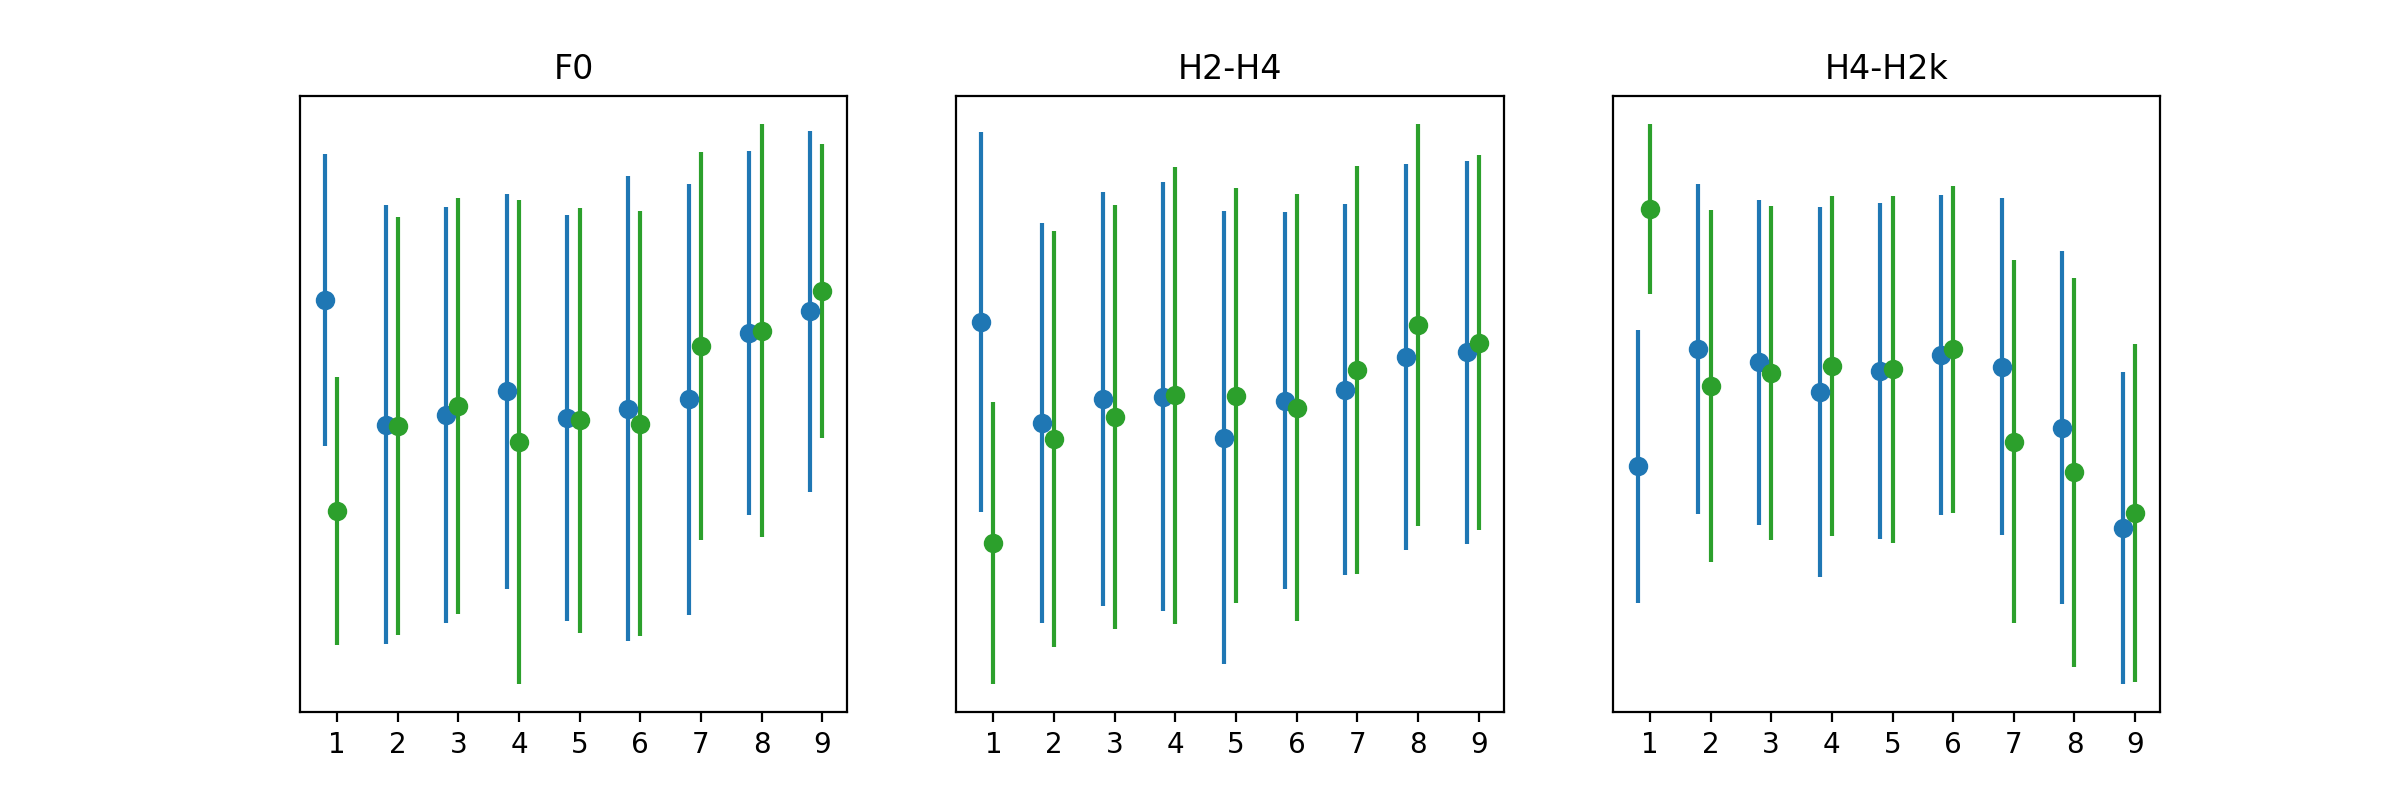
\includegraphics[width=\linewidth]{IS2019_paper_kit/images/errbar_VQual_clstr_flase.png}
%     \caption{\label{fig:vqual}Caption}
% \end{figure}


\subsection{Mel-Frequency Cepstral Coefficients}

Mel-frequency cepstral coefficients (MFCCs) are widely used acoustic features in speech processing.  %This feature set represents the overall spectral envelope of speech signals. , and is closely related to the vocal tract shape. Physiological changes due to sleepiness might shape the vocal tract in a certain way that can be reflected in the spectral envelope. Thus, the distribution of MFCCs over an utterance might provide information about the degree of sleepiness of the speaker.
MFCCs were extracted with a window size of 25 ms, a window shift of 10 ms, a pre-emphasis filter with coefficient 0.97, and a sinusoidal lifter with coefficient 22. A filter bank with 23 filters was applied and 13 coefficients were extracted. 
The first and the second derivatives were also used. %The voice box toolkit was used to extract MFCC features~\cite{brookes1997voicebox}.

\subsection{Entropy}

Between-frame entropy was calculated as described in~\cite{you2004entropy}. MFCCs were obtained from the speech signal using a Hamming window of length 25 ms and a frame shift of 2.5 ms. A 30 ms rectangular window was applied to MFCCs and using the features in this window, the signal's local entropy was computed as:

\begin{equation}
    H(v) = K \ln{\sqrt{2\pi}} + \ln{\Tr({\Sigma})},
\end{equation}
where, $H(v)$ is the entropy of the random variable $v$ of dimension $K$ and $\Sigma$ is the $ K \times K $ covariance matrix of the probability distribution function of the random variable $v$.  

%If an acoustic feature changes rapidly, the entropy of an acoustic feature between frames would be high. 
%\Soo{I wrote this para without a crystal clear idea about the entropy we are using. Please read this section and correct if needed}
The spectral variability of the speech signal is represented by entropy. Rapid information gain in the speech spectrum corresponds to high entropy. Hence, we expected between-frame entropy to correlate with instantaneous speech rate. In order to verify this hypothesis, the correlation between the number of syllables per second, a conventional speech rate measure, and the mean between-frame entropy within an utterance was calculated. Syllables per second were computed using a Praat script as described in \cite{DeJong2009}.

The computed speech rate was highly correlated with the mean frame-level change in entropy for the training data, as shown in Figure~\ref{fig:entropy_rate}. The linear regression between the mean of speech rate and the mean of entropy resulted in $R^2=0.50$ and $p<0.001$.  The corresponding Pearson's correlation coefficient was 0.71. The high correlation provides evidence to the hypothesis that between-frame entropy can be used to represent speech rate.
The unexplained variance in the linear regression might be due to the difference in information reflected in each methods.
For example, the syllables per second measure only focuses on syllable nuclei, while the between-frame entropy changes over all frames in an utterance.
%Another possibility is in unexpected inaccuracies in the entropy and/or speech rate calculation algorithms. 


%While speech rate in terms of the number of syllables per second or words per minute can be calculated at the utterance level, entropy can be calculated frame by frame. The distribution of instantaneous speech rate might provide more information about sleepiness of the speaker than the average speech rate over an utterance. %Experimental results verified this hypothesis. 

\begin{figure}
    \centering
    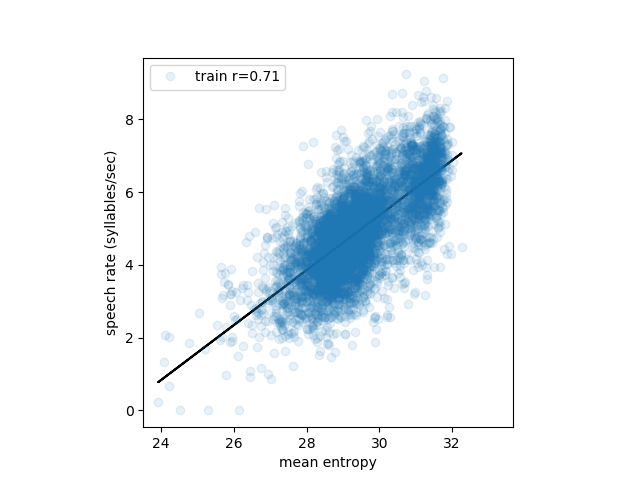
\includegraphics[width=\linewidth]{IS2019_paper_kit/images/scatter_train.png}
    \caption{\label{fig:entropy_rate}Scatter plot of speech rate in terms of syllables per second vs. mean of frame level change in entropy within an utterance in the training dataset. A line was fitted using linear regression ($R^2=0.50$, $p<0.001$).}
\end{figure}

\subsection{ComParE16 Feature Set}

%\Soo{Maybe we can mention that this feature set is considered as the baseline feature set}
This feature set is provided as the baseline of the Interspeech 2019 Continuous Sleepiness sub-challenge. The ComParE16 feature set~\cite{weninger2013acoustics} consists of $F_0$, energy, spectral, cepstral and voicing related frame-level features. Additionally, the set includes the zero crossing rate, jitter, shimmer, harmonic-to-noise ratio (HNR), spectral harmonicity and psychoacoustic spectral sharpness. These are referred to as low-level descriptors (LLDs). The OpenSMILE toolkit was used to extract the ComParE16 features~\cite{eyben2010opensmile}.



%\Soo{These are not LLDs?}. This feature set comprises of 6,373 static features resulting from the computation of various functionals
%\Soo{`functionals' means the statistics vectors? Any utterance representation should be described in 4.1.2} 
%over low-level descriptor contours. The functionals used are statistical functions, polynomial regression coefficients and transformations on the low-level descriptors. 
\subsection{Utterance Representation}
%\subsubsection{i-vector}
  
Two types of utterance representations were used in this study.
First, the i-vector was used to represent the distribution of frame-level acoustic features. A universal background model (UBM, \cite{Reynolds2000}) with 2,048 Gaussian mixtures and a 600-dimensional i-vector extractor was trained using SRE and Switchboard databases. Speech signals in the SLEEP database were downsampled to a sampling rate of 8~kHz to match the bandwidth of the training databases prior to i-vector extraction. %The i-vector representation was used for MFCCs and VQual features.                                  

%\subsubsection{Statistics Vector}
%which statistics

Second, 
%We also provide a comparison of the performance of our system using i-vector representation of utterances against the performance of the same system using a statistics vector representation. 
the statistics vector was used as a baseline utterance representation that maps the contours of the acoustic features onto a fixed dimensionality vector. Peaks, percentiles, moments, regression, temporal and modulation functionals were computed \cite{weninger2013acoustics}. The OpenSmile toolkit \cite{eyben2010opensmile} was used to compute the statistics vector. %The statistics vector representation was used for  ComParE16, MFCCs, VQual and between-frames changes in entropy. %Mulitlevel Prediction

% =====================================
\section{Sleepiness Prediction}
% =====================================

\subsection{Utterance Representation}
\subsubsection{i-vector}
  
A universal background model (UBM, \cite{dehak2011front}) with 2048 Gaussian mixtures and a 600-dimensional i-vector extractor was trained using the SRE and the Switchboard databases. Speech signals in the SLEEP database were downsampled to a sampling rate of 8 kHz to match the bandwidth of the SRE and Switchboard databases for i-vector extraction. The i-vector representation was used for MFCCs and VQual features.                                  

\subsubsection{Statistics Vector}
%which statistics

%We also provide a comparison of the performance of our system using i-vector representation of utterances against the performance of the same system using a statistics vector representation. 
The statistics vector was used as a baseline utterance representation that maps the contours of the acoustic features onto a fixed dimensionality vector. Peaks, percentiles, moments, regression, temporal and modulation functionals were computed \cite{weninger2013acoustics}. The OpenSmile toolkit \cite{eyben2010opensmile} was used to compute the statistics vector. The statistics vector representation was used for  ComParE16, MFCCs, VQual and between-frames changes in entropy.


\subsection{Data Processing}

The training data was processed by eliminating the outliers prior to training the predictor. We used the Elliptic Envelope outlier detection algorithm with a contamination value of 15\%. The outlier detection system was trained on i-vector representation of between-frame changes in entropy. The contamination value was optimized for maximized performance on the development set. The effectiveness of the outlier detection system was tested by training the predictor with and without data processing. 




\subsection{System Description}

In this experiment, we used the support vector machines regressor (SVR) to predict the sleepiness degree. The complexity parameter of the predictor, $C$, was chosen from a range of values between $10^{-6}$ and $10^{5}$ so as to maximize the system performance on the development dataset. Experiments were performed to compare the two types of utterance representation- i-vector and statistics vector using the feature sets described earlier. The same set of experiments were done with and without processing the training data prior to training the predictor. 

Instead of the feature concatenation, we performed a score level fusion using individual features. The final prediction was a linear combination of predictions obtained from individual features. The weights for the linear combination are determined by a grid search. 


 
 \Soo{Provide an explanation for the outlier detection module}


\iffalse
\subsection{Multi-Level System}

Assessing the sleepiness of speakers as a regression problem is a challenging task since there are a total of 9 possible prediction labels with a considerable imbalance in training data for each label. As can be seen from Table \ref{tab:KSS}, rating 1 and 9 have less than half as many utterances compared to rating 3. To alleviate this data imbalance problem, we propose a multilevel prediction strategy: a 3-class classification and a regression within each class. 

\subsubsection{Level 1: Classification}

In the first level, each utterance is  classified into three classes. The classes represent low, moderate and high degrees of sleepiness. The KSS ratings of 1, 2, and 3 were considered as low;  4, 5, and 6 as moderate degrees of sleepiness and ratings 7, 8, and 9 as high degrees of sleepiness. 
A support vector classifier (SVC) using a radial basis function (RBF) kernel implemented in the Sklearn library was used. Similar to the single level system, the complexity parameter $C_2$ was optimized.

\subsubsection{Level 2: Regression}
For each of the three classes (low, moderate and high levels of sleepiness), a regressor was used to predict the KSS rating of each utterance. In this second level, a support vector regressor (SVR) from Sklearn was used. Again, the complexity parameter $C_3$
was optimized for maximum system performance on the development dataset for both feature sets. Score fusion was performed on two second-level systems- one developed using the voice quality features and the other, using the MFCC features. 
\fi

\subsection{Evaluation Metric}

The task in this challenge is to assess the sleepiness of a speaker as a regression problem. Spearman's correlation coefficient ($\rho$) was used for performance evaluation \cite{schullerinterspeech}. 
Spearman's correlation coefficient was selected among various correlation measures because it is robust. For example, the Pearson correlation coefficient measures the strength of linear relationships between the normally distributed variables ~\cite{hauke2011comparison}, but the predictions in our experiments may neither be normally distributed nor have a linear relationship.  %Experimental Results
% =====================================
\section{Experimental Results}
% ============

\subsection{Single-Level System Performance}

System performance without outlier detection is first analyzed. A comparison of the effectiveness of the statistics vector and i-vector utterance representations is presented in Table \ref{tab:results_single_level_system}. The baseline system used ComParE16 feature set.

\begin{table}[h]
\centering

\caption{\label{tab:results_single_level_system}Correlation results for the development set without data processing. The best performing combination is boldfaced.}

\begin{tabular*}{\linewidth}{l@{\extracolsep{\fill}}lc}
\toprule
\textbf{Utt. representation} & \textbf{Feature set} & \textbf{ $\rho$} \\
\midrule
\midrule

\multirow{4}{*}{Statistics vector} 
% & ComParE16 & \textbf{0.251} \\
& entropy & 0.029 \\
& VQual & 0.142 \\
& MFCC & 0.158 \\
 \midrule
\multirow{3}{*}{i-vector}
& entropy & 0.126\\
& VQual & 0.201 \\
 & MFCC & \textbf{0.248} \\
 \bottomrule
\end{tabular*}%

\end{table}





Using the i-vector framework improved system performance substantially compared to using statistics vectors when the same acoustic features were used. 
For example, when MFCCs were used, the performance improved from 0.158 to 0.248, a relative improvement of approximately 56\%. When VQual features were used the, improvement was around 40\%, from a $\rho$ value of 0.142 to 0.201. This improvement could partially be due to the compensation of speaker and phonetic variability.


\begin{table}[h]
\centering

\caption{\label{tab:results_single_level_system}Correlation results for the development set with data processing. The best performing combination is boldfaced.}

\begin{tabular*}{\linewidth}{l@{\extracolsep{\fill}}lc}
\toprule
\textbf{Utt. representation} & \textbf{Feature set} & \textbf{ $\rho$} \\
\midrule
\midrule

\multirow{4}{*}{Statistics vector} 
% & ComParE16 &  \textbf{0.271}\\
& entropy & 0.078 \\
& VQual &  0.179\\
& MFCC &  0.192\\
 \midrule
\multirow{3}{*}{i-vector}
& entropy & 0.131\\
& VQual &  0.221\\
 & MFCC &  \textbf{0.252}\\
 \bottomrule
\end{tabular*}%

\end{table}

 




 The performance of a fused system was better than individual systems for both types of utterance representations. When statistics vectors were used, the score level fusion of MFCC and VQual improved the $\rho$ value from 0.158 for MFCC alone to 0.182 for the fusion system (15\% relative improvement). In case of ComParE16 features, fusing with VQual improved the $\rho$ value from 0.251 to 0.261. When i-vectors were used, the improvement in $\rho$ was from 0.248 for MFCC alone to 0.265 for the fused system (6\% relative improvement). This performance improvement with score level fusion can be explained with the complimentary nature of the feature sets. We do not report score fusion for other features since no improvement in performance was observed. We observe that across features, fusing with VQual improves results. 

 When between-frame changes in entropy is used in the single-level system the system performance is low. This might be potentially due the reason that 
 \Soo{You can refer to \cite{Vogel2011} that speech rate had opposite pattern between read and spontaneous speech}



\begin{table}[t]
\centering

\caption{\label{tab:outlier_results}Correlation results for the development set with data processing and score fusion. Statistics vector representation for ComParE feature set and i-vector representation for MFCCs and VQual were used. The `+' sign indicates score level fusion. The best performing combination is boldfaced.}

\begin{tabular*}{\linewidth}{l@{\extracolsep{\fill}}l}
\toprule
\textbf{Feature sets} & \textbf{ $\rho$} \\
\midrule
\midrule

ComParE16+VQual & 0.283\\
\addlinespace
ComParE16+MFCCs & 0.296\\
\addlinespace
ComParE16+MFCCs+VQual &\textbf{0.300} \\
\addlinespace
 \bottomrule
\end{tabular*}%

\end{table}

\subsection{Mulit-Level System Performance}
%We further build upon the single level system by implementing a multi-level system that predicts the sleepiness degree by first classifying the utterance and then doing a regression. 
The multi-level prediction method was implemented using only the i-vector utterance representation since the overall performance of the system using i-vectors is better than those using statistics vectors. 
Multi-level prediction results are shown in Table \ref{tab:results_multi_level_system}. 

Three different combinations of features were tested to implement the prediction. Each feature set -- entropy, Voice Quality and MFCC was used for classification (level 1) and the other two feature sets were used for regression, followed by a score fusion (level 2). The system performance was best when entropy is used for classification and MFCC and VQual were used for regression. 

Interestingly, although entropy did not perform better than other features for single-level prediction, it provided a performance gain when it was used for the classification followed by the regression using other feature sets. 

In brief, the best performing system was the one which used between-frame changes in entropy for classification followed by regression on VQual and MFCC with score level fusion. With a Spearman's correlation coefficient of 0.269,  our final system was able to achieve a relative improvement of 7.17\% over the baseline. 
The ComParE 2016 feature set provided with the baseline system had a $\rho$ of 0.251. 
% The confusion matrix for this is shown in Figure \ref{fig:}.  \Vijay{discussion on confusion matrix}

Speaker and phonetic variability poses a challenge to speaker state recognition~\cite{pisoni1989effects}. These may affect the acoustic variability arising due to the degree of sleepiness of a speaker thereby reducing the performance of sleepiness prediction systems. Bone~\etal~\cite{bone2011intoxicated} suggested the use speaker normalization to detect intoxicated speech.

\begin{table}[t]
\centering

\caption{\label{tab:outlier_results}Correlation results for the test set with data processing and score fusion. Statistics vector representation for ComParE feature set and i-vector representation for MFCCs and VQual were used. The `+' sign indicates score level fusion. the baseline system used ComParE16 feature set, as shown in the first row}

\begin{tabular*}{\linewidth}{l@{\extracolsep{\fill}}l}
\toprule
\textbf{Feature sets} & \textbf{ $\rho$} \\
\midrule
\midrule

ComParE16 & 0.314\\
\addlinespace
ComParE16+MFCCs+VQual & \\
\addlinespace
 \bottomrule
\end{tabular*}%

\end{table} %Conclusion
% =====================================
\section{Conclusion}
% =====================================
This study proposes the use of voice quality features (VQual) and between-frames changes in entropy for the prediction of sleepiness degree. VQual features are related to the perceived voice quality, and changes in entropy are an indirect measure of speech rate. An i-vector system was employed to reduce speaker and phonetic variability. To address the challenge of data imbalance, a multi-level prediction system was developed. A score-level fusion was done on complimentary features. 

In the single-level system, we observed a substantial gain in system performance when voice quality features were fused. In the case of multi-level system, the system performance was better when between-frame changes in entropy were used. Thus, the proposed acoustic feature set improved the performance of sleepiness prediction system. The i-vector system was an effective representation of the utterance. By implementing the i-vector representation for an utterance, we reduced variability in data arising due to factors extrinsic to speaker's degree of sleepiness. The resulted in a considerable improvement in system performance.  

Since the UBM was trained on an English database, it will be interesting in the future to develop a UBM on a German speech database. Developing an i-vector utterance representation for the ComParE16 features will be another important future study. 
 %Conclusion




%\section{Acknowledgements}
% \section{References}

\bibliographystyle{IEEEtran}

\bibliography{references}

% \begin{thebibliography}{9}
% \bibitem[1]{Davis80-COP}
%   S.\ B.\ Davis and P.\ Mermelstein,
%   ``Comparison of parametric representation for monosyllabic word recognition in continuously spoken sentences,''
%   \textit{IEEE Transactions on Acoustics, Speech and Signal Processing}, vol.~28, no.~4, pp.~357--366, 1980.
% \bibitem[2]{Rabiner89-ATO}
%   L.\ R.\ Rabiner,
%   ``A tutorial on hidden Markov models and selected applications in speech recognition,''
%   \textit{Proceedings of the IEEE}, vol.~77, no.~2, pp.~257-286, 1989.
% \bibitem[3]{Hastie09-TEO}
%   T.\ Hastie, R.\ Tibshirani, and J.\ Friedman,
%   \textit{The Elements of Statistical Learning -- Data Mining, Inference, and Prediction}.
%   New York: Springer, 2009.
% \bibitem[4]{YourName17-XXX}
%   F.\ Lastname1, F.\ Lastname2, and F.\ Lastname3,
%   ``Title of your INTERSPEECH 2019 publication,''
%   in \textit{Interspeech 2019 -- 20\textsuperscript{th} Annual Conference of the International Speech Communication Association, September 15-19, Graz, Austria, Proceedings, Proceedings}, 2019, pp.~100--104.
% \end{thebibliography}

\end{document}
